\graphicspath{{Chapter1/Figs/}}

\chapter{Joint profiling of chromatin accessibility DNA methylation and transcription in single cells}

In this Chapter I describe scNMT-seq, an experimental protocol for genome-wide profiling of RNA expression, DNA methylation and chromatin accessibility in single cells. First, I show a validation of the quality of the molecular readouts, including a comparison with existing technologies. Subsequently, I showcase how scNMT-seq can be used to reveal coordinated epigenetic and transcriptomic heterogeneity along a differentiation process.

The work discussed in this Chapter results from a collaboration with the group of Wolf Reik (Babraham Institute, Cambridge, UK). It has been peer-reviewed and published in \cite{Clark2018}. The methodology was conceived by Stephen Clark, who performed most of the experiments. Felix Krueger processed and managed sequencing data. I performed all the computational analysis shown in this chapter. John C. Marioni, Oliver Stegle and Wolf Reik supervised the project. The article was jointly written by Stephen Clark and me, with input from all authors.

\section{Description of the experimental protocol} \label{section:scnmt_protocol}

scNMT-seq builds upon two previous multi-modal protocols: single-cell Methylation and Transcriptome sequencing (scM\&T-seq) \cite{Angermueller2016} and Nucleosome Occupancy and Methylation sequencing (NOMe-seq) \cite{Kelly2012,Pott2016}. An overview of the protocol is shown in \Cref{fig:scnmt_protocol}.

In the first step (the NOMe-seq step), cells are sorted into individual wells and incubated with a GpC methyltransferase (M.CviPI). This enzyme labels accessible (or nucleosome depleted) GpC sites via DNA methylation\cite{Kilgore2007, Kelly2012}. In mammalian genomes, cytosine residues in GpC dinucleotides are methylated at a very low rate. Hence, after M.CviPI treatment, GpC methylation marks can be interpreted as direct read outs for chromatin accessibility, as opposed to the CpG methylation readouts, which can be interpreted as endogenous DNA methylation\cite{Kilgore2007, Kelly2012}.

In a second step (the scM\&T-seq step), the DNA molecules are separated from the mRNA using oligo-dT probes pre-annealed to magnetic beads. Subsequently, the DNA fraction undergoes single-cell bisulfite conversion\cite{Smallwood2014}, whereas the RNA fraction undergoes Smart-seq2 \cite{Picelli2014}.\\

\begin{figure}[H]
	\centering
	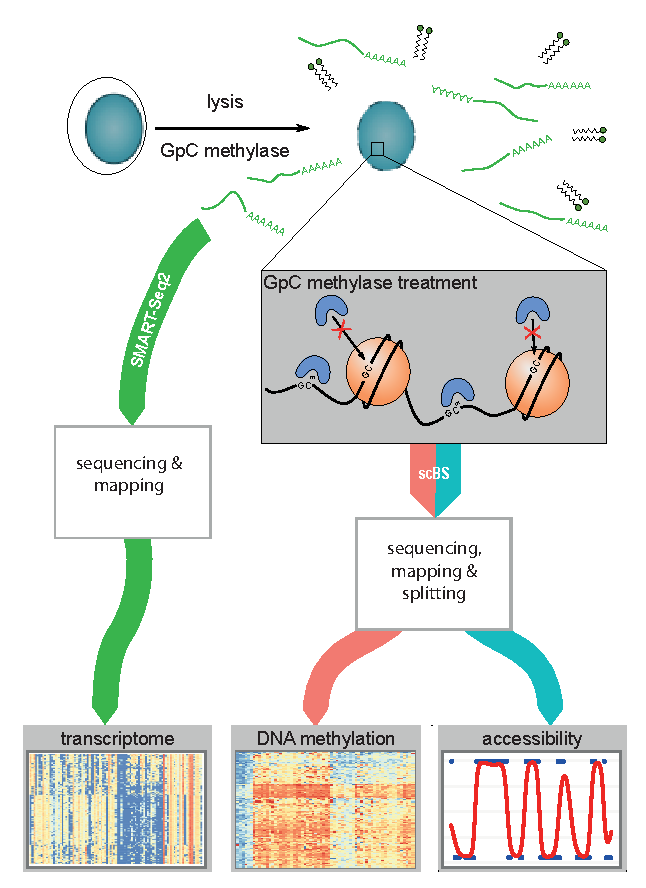
\includegraphics[width=0.55\linewidth]{scNMT_protocol}
	\caption[]{\textbf{scNMT-seq protocol overview.}\\
	In the first step, cells are isolated and lysed. Second, cells are incubated with a GpC methyltransferase. Third, the RNA fraction is separated using oligo-dT probes and sequenced using Smart-seq2. The DNA fraction undergoes scBS-seq library preparation and sequencing. Finally, CpG Methylation and GpC chromatin accessibility data are separated computationally.}
	\label{fig:scnmt_protocol}
\end{figure}

As discussed in \Cref{section:chromatin_accessibility}, NOMe-seq has a range of appealing properties in comparison with count-based methods such as ATAC-seq or DNAseq-seq. First, the obvious gain of simultaneously measuring another epigenetic readout such as DNA methylation with little additional cost. Second, the resolution of the method is determined by the frequency of GpC sites within the genome ($\approx$ 1 in 16 bp), rather than the size of a library fragment (usually >100 bp). This allows the robust inspection of individual regulatory elements, nucleosome positioning and transcription factor footprints \cite{Kelly2012,Pott2016,Nordstrom2019}. Third, missing data can be easily discriminated from inaccessible chromatin. Importantly, this implies that lowly accessible sites will not suffer from increased technical variation (due to low read counts) compared to highly accessible sites. Finally, the M.CviPI enzyme shows less sequence motif biases than the DNAse or the Tn5 transposase \cite{Nordstrom2019}.

The downsides of the approach are the limited scalability associated with plate-based methods, and the need to discard read outs from (1) GCG positions (21\% of all CpG sites), as it is intrinsically not possible to distinguish endogenous methylation from \textit{in vitro} methylated bases, and (2) CGC positions (27\%), to mitigate off-target effects of the enzyme \cite{Kelly2012}. This filtering step reduces the number of genome-wide cytosines that can be assayed from 22 million to 11 million. 


\section{Description of the data processing pipeline}

After DNA sequencing, reads undergo quality control and trimming using TrimGalore to remove the flanking 6bp (the random primers), adaptor contamination and poor-quality base calls. Subsequently, trimmed reads are aligned to the corresponding genome assembly. Here we used Bismark \cite{Krueger2011} with the additional --NOMe option, which produces CpG report files containing only ACG and TCG trinucleotides and GpC report files containing only GCA, GCC and GCT positions.

Following \cite{Smallwood2014}, a bernoulli model is assumed for each CpG and GpC site in each cell after removal of duplicate alignments, which results in binary methylation calls. Notice that the use of a bernoulli model is an exclusive property of single-cell bisulfite sequencing data, for the vast majority of sites only one allele is observed per cell (due to data sparsity). This contrasts with bulk bisulfite sequencing data, where each dinucleotide typically contains multiple reads (originating from different cells) and thus a binomial model is more appropriate than a bernoulli estimate.

Finally, when quantifying DNA methylation and chromatin accessibility over genomic features (i.e. promoters or enhancers) a binomial model is assumed for each cell and feature, where the number of successes is the number of methylated CpGs (or GpCs) and the number of trials is the total number of CpGs (or GpCs) that are observed within the specific cell and genomic feature.

\section{Data validation}

\subsection{Coverage} \label{section:scnmt_coverage}

We validated scNMT-seq in 70 EL16 mouse embryonic stem cells (ESCs), together with 3 cells processed without M.CviPI enzyme treatment (i.e. using scM\&T-seq). The use of this relatively simple and well-studied \textit{in vitro} system allows us to compare our DNA methylation and chromatin accessibility statistics to published data \cite{Smallwood2014,Angermueller2016,Ficz2013}.

First, we compared the theoretical maximum coverage that could be achieved with the empirical coverage (\Cref{fig:scnmt_coverage}). Despite the reduction in theoretical coverage due to the removal of ambiguous CCG and GCG sites, we observed, for DNA methylation, a median of $\approx$ 50\% of promoters, $\approx$ 75\% of gene bodies and $\approx$ 25\% of active enhancers captured by at least 5 CpGs in each cell. Nevertheless, limited coverage is indeed observed for small genomic contexts such as p300 ChIP-seq peaks (median of $\approx$ 200bp).\\
For chromatin accessibility, coverage was larger than that observed for endogenous methylation due to the higher frequency of GpC dinucleotides, with a median of $\approx$ 85\% of gene bodies and $\approx$ 75\% of promoters measured with at least 5 GpCs.

\begin{figure}[H]
	\centering
	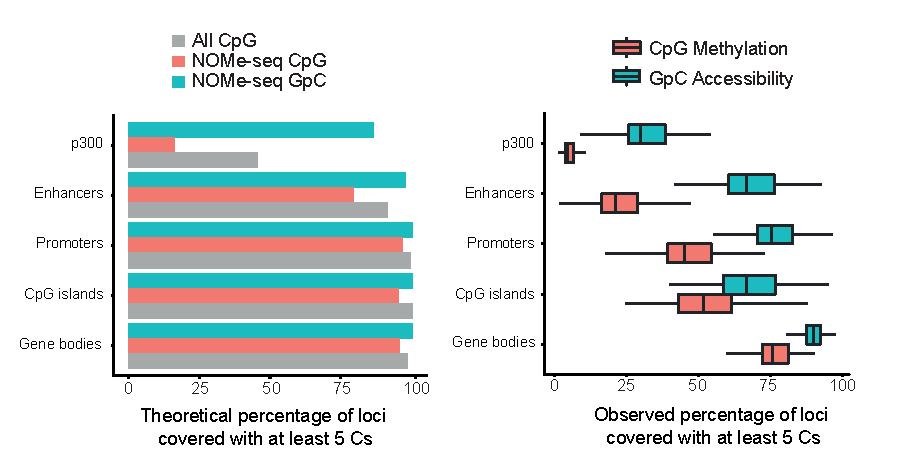
\includegraphics[width=1.0\linewidth]{scNMT_coverage}
	\caption[]{\textbf{Coverage statistics for CpG DNA methylation and GpC chromatin accessibility}.\\ 
	(a) Fraction of loci with at least 5 CpG (red) or GpC (blue) dinucleotides per genomic context, after exclusion of the conflicting trinucleotides. The grey bar shows the total number of CpGs without exclusion of trinucleotides. (b) Empirical coverage per genomic context in a data set of 61 mouse ES cells. The empirical coverage is quantified as the fraction of loci with at least 5 CpG (red) or GpC (blue) observed. The boxplots summarise the distribution across cells, showing the median and the 1st and 3rd quartiles.}
	\label{fig:scnmt_coverage}
\end{figure}

Next, we compared the DNA methylation coverage with a similar data set profiled by scM\&T-seq \cite{Angermueller2016} (\Cref{fig:scnmt_coverage2}), where the the conflicting trinucleotides are not excluded.\\
Despite scNMT-seq yielding less CpG measurements, we find little differences in coverage when quantifying DNA methylation over genomic contexts, albeit these become evident when down-sampling the number of reads.

\begin{figure}[H]
	\centering
	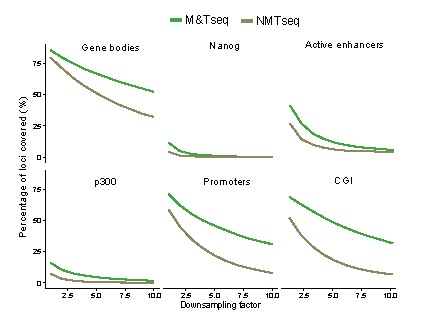
\includegraphics[width=0.8\linewidth]{scNMT_coverage2}
	\caption[]{\textbf{Comparison of the empirical coverage of DNA methylation with scM\&T-seq \cite{Angermueller2016}}.\\
	The y-axis displays the fraction of loci covered with at least 5 CpG sites. The x-axis displays the downsampling factor, where the value of 1 corresponds to no downsampling (i.e. the base line). To facilitate the comparison, we selected two cells that were sequenced at equivalent depth.}
	\label{fig:scnmt_coverage2}
\end{figure}

\subsection{Consistency with previous studies}

To assess the consistency with previous studies we quantified DNA methylation and chromatin accessibility using a running window throughout the genome. The resulting methylomes were compared to datasets from the same cell lines profiled with similar technologies, including scM\&T-seq\cite{Angermueller2016}, scBS-seq\cite{Smallwood2014} and bulk BS-seq\cite{Ficz2013}. We find that most of the variation is not attributed to the technology but to differences in culture condition (\Cref{fig:scnmt_comparison}). This result is expected, as cells grown in 2i media remain in a native pluripotency state that is associated with genome-wide DNA hypomethylation \cite{Ficz2013}. Interestingly, the serum-cultured cells processed in this study overlapped with 2i-cultured cells from previous datasets. suggesting that they remained in a more pluripotent state. The most likely explanation for this variation is the differences in the cell lines (we used female EL16 versus male E14 in \cite{Angermueller2016,Smallwood2014,Ficz2013}). Previous studies have shown that female ESCs tend to show lower levels of mean global methylation, which is consistent with a more pluripotent phenotype \cite{Zvetkova2005}.\\

In terms of accessibility, no NOMe-seq measurements were available for ESCs at the time of the study, so we compared it to bulk DNase-seq data from the same cell type, yielding good consistency between datasets ($R=0.74$).
\begin{figure}[H]
	\centering
	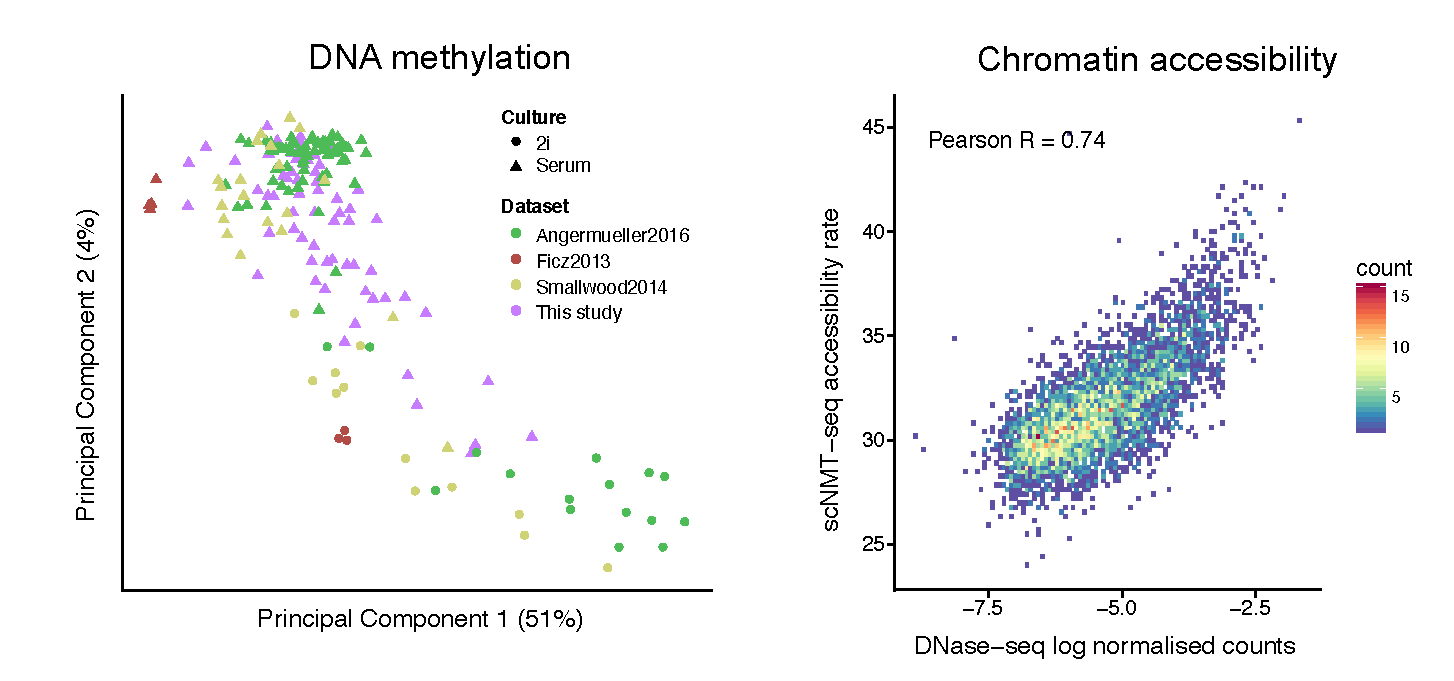
\includegraphics[width=1.0\linewidth]{scNMT_comparison}
	\caption[]{\textbf{Comparison of unsupervised genome-wide quantifications to published datasets}.\\
	(a) Principal Component Analysis of 1kb running windows. Missing values were imputed using the average methylation rate per locus.\\
	(b) Scatter plot of chromatin accessibility quantified over 10kb running windows of scNMT-seq data versus published bulk DNase-seq. For DNase-seq, accessibility is quantified as the log2 reads. The Pearson correlation was weighted by the GpC coverage in scNMT-seq data. }
	\label{fig:scnmt_comparison}
\end{figure}


\subsection{Quantification of DNA methylation and chromatin accessibility in known regulatory regions}

We pseudobulked the data across all cells and examined DNA methylation and chromatin accessibility levels at loci with known regulatory roles. We found that in CTCF binding sites and DNaseI hypersensitivity sites DNA methylation was decreased while chromatin accessibility was increased, as previously reported \cite{Pott2016}. As a control, we observe that cells which did not receive M.CviPI treatment showed globally low GpC methylation levels ( $\approx$ 2\%, \Cref{fig:scnmt_pseudobulk_profiles}).

\begin{figure}[H]
	\centering
	\includegraphics[width=0.7\linewidth]{scnmt_pseudobulk_profiles}
	\caption[]{\textbf{Accessibility and methylation profiles in regulatory genomic contexts.}\\
	First, we pseudobulk the data set by pooling information across all cells. Next, we compute running averages of the CpG methylation (red) and the GpC accessibility (blue) in consecutive non-overlapping 50bp windows. Solid line displays the mean across all genomic elements within a given annotation and the shading displays the corresponding standard deviation.\\
	(a) Profiles for scNMT-seq cells. (b) Profiles for scMT-seq cells
	}
	\label{fig:scnmt_pseudobulk_profiles}
\end{figure}

\subsection{Quantification of the association between molecular layers.}

We attempted to reconstruct the expected directional relationships between the transcriptome and the epigenome, namely the positive association between RNA expression and chromatin accessibility and the negative association between DNA methylation and RNA expression \cite{Thurman2012,Angermueller2016}.\\
To get a measure of the association (or coupling) between two molecular layers, we quantified a linear association per cell (across genes). Notice that this approach is not exclusive to single-cell data and can also be computed (more accurately) with bulk measurements. Reassuringly, this analysis confirmed, even within single cells, the expected positive correlation between chromatin accessibility and RNA expression, and the negative correlations between RNA expression and DNA methylation, and between DNA methylation and chromatin accessibility.

\begin{figure}[H]
	\centering
	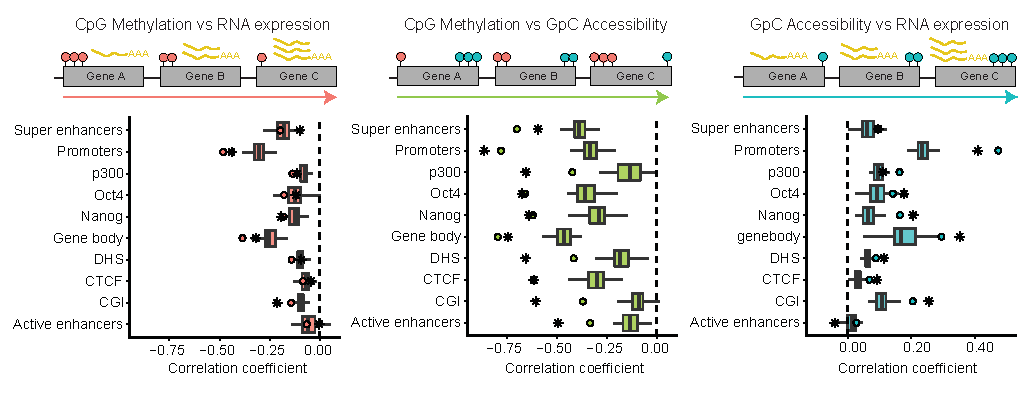
\includegraphics[width=1.0\linewidth]{scNMT_correlations_acrossgenes}
	\caption[]{\textbf{Quantification of linear associations between molecular layers.}\\
	The top diagram illustrates the computation of an association test per cell (across all loci in a given genomic context). The left panel shows DNA methylation versus RNA expression. The middle panel shows DNA methylation versus chromatin accessibility. The right panel shows RNA expression versus chromatin accessibility. The x-axis displays the Pearson correlation coefficients between two molecular layers, per genomic context (y-axis). The box plots summarise the distribution of correlation coefficients across cells. The dots and stars show the linear associations quantified in pseudo-bulked scNMT-seq data and published bulk data from the same cell types \cite{Ficz2013,ENCODE2012}, respectively. }
	\label{fig:scNMT_correlations_acrossgenes}
\end{figure}

% Consistently, when stratifiying the loci from \Cref{fig:scnmt_profiles} based on the expression level of the nearest gene, we observe that higher RNA expression is associated with chromatin openness and decreased DNA methylation levels \Cref{fig:scnmt_profiles_byexpr}. 
% \begin{figure}[H]
% 	\centering
% 	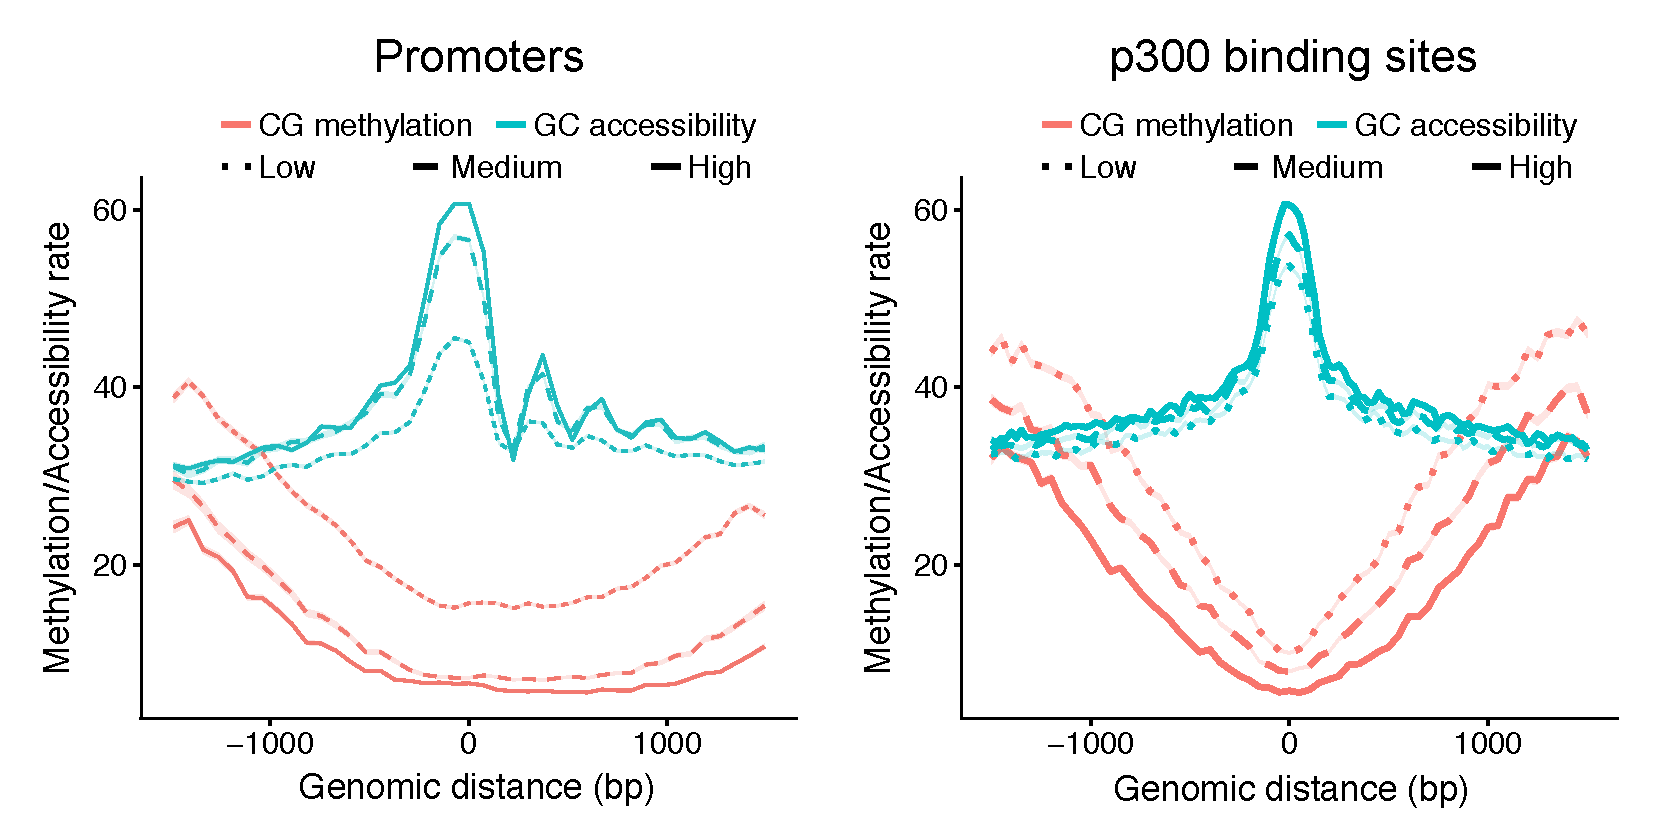
\includegraphics[width=0.9\linewidth]{scNMT_pseudobulk_profiles_byexpr}
% 	\caption[]{DNA methylation (red) and chromatin accessibility profiles (blue), stratified by RNA expression of the nearest gene. The profiles are quantified as in \Cref{fig:scnmt_profiles}. The RNA expression is discretised in three groups: log normalised counts less than 2 (low), between 2 and 6 (medium) and higher than 5 (high)}
% 	\label{fig:scnmt_profiles_byexpr}
% \end{figure}


\section{Application to an embryoid body differentiation data set}

\subsection{Identification of genomic elements with coordinated variability across molecular layers}

Having validated the quality of scNMT-seq data with a simple and relatively homogeneous data set, we next explored its potential to identify coordinated heterogeneity between the transcriptome and the epigenome.\\
We generated a second data set of 43 embryonic stem cells (after quality control), where we induced a differentiation process towards embryoid bodies by removing the LIF media for 3 days.\\Dimensionality reduction on the RNA expression data reveals the existence of two subpopulations: one with high expression of pluripotency markers (\textit{Esrrb} and \textit{Rex1}) and the other with high expression of differentiation markers (\textit{T} and \textit{Prtg}).

% \begin{figure}[H]
% 	\centering
% 	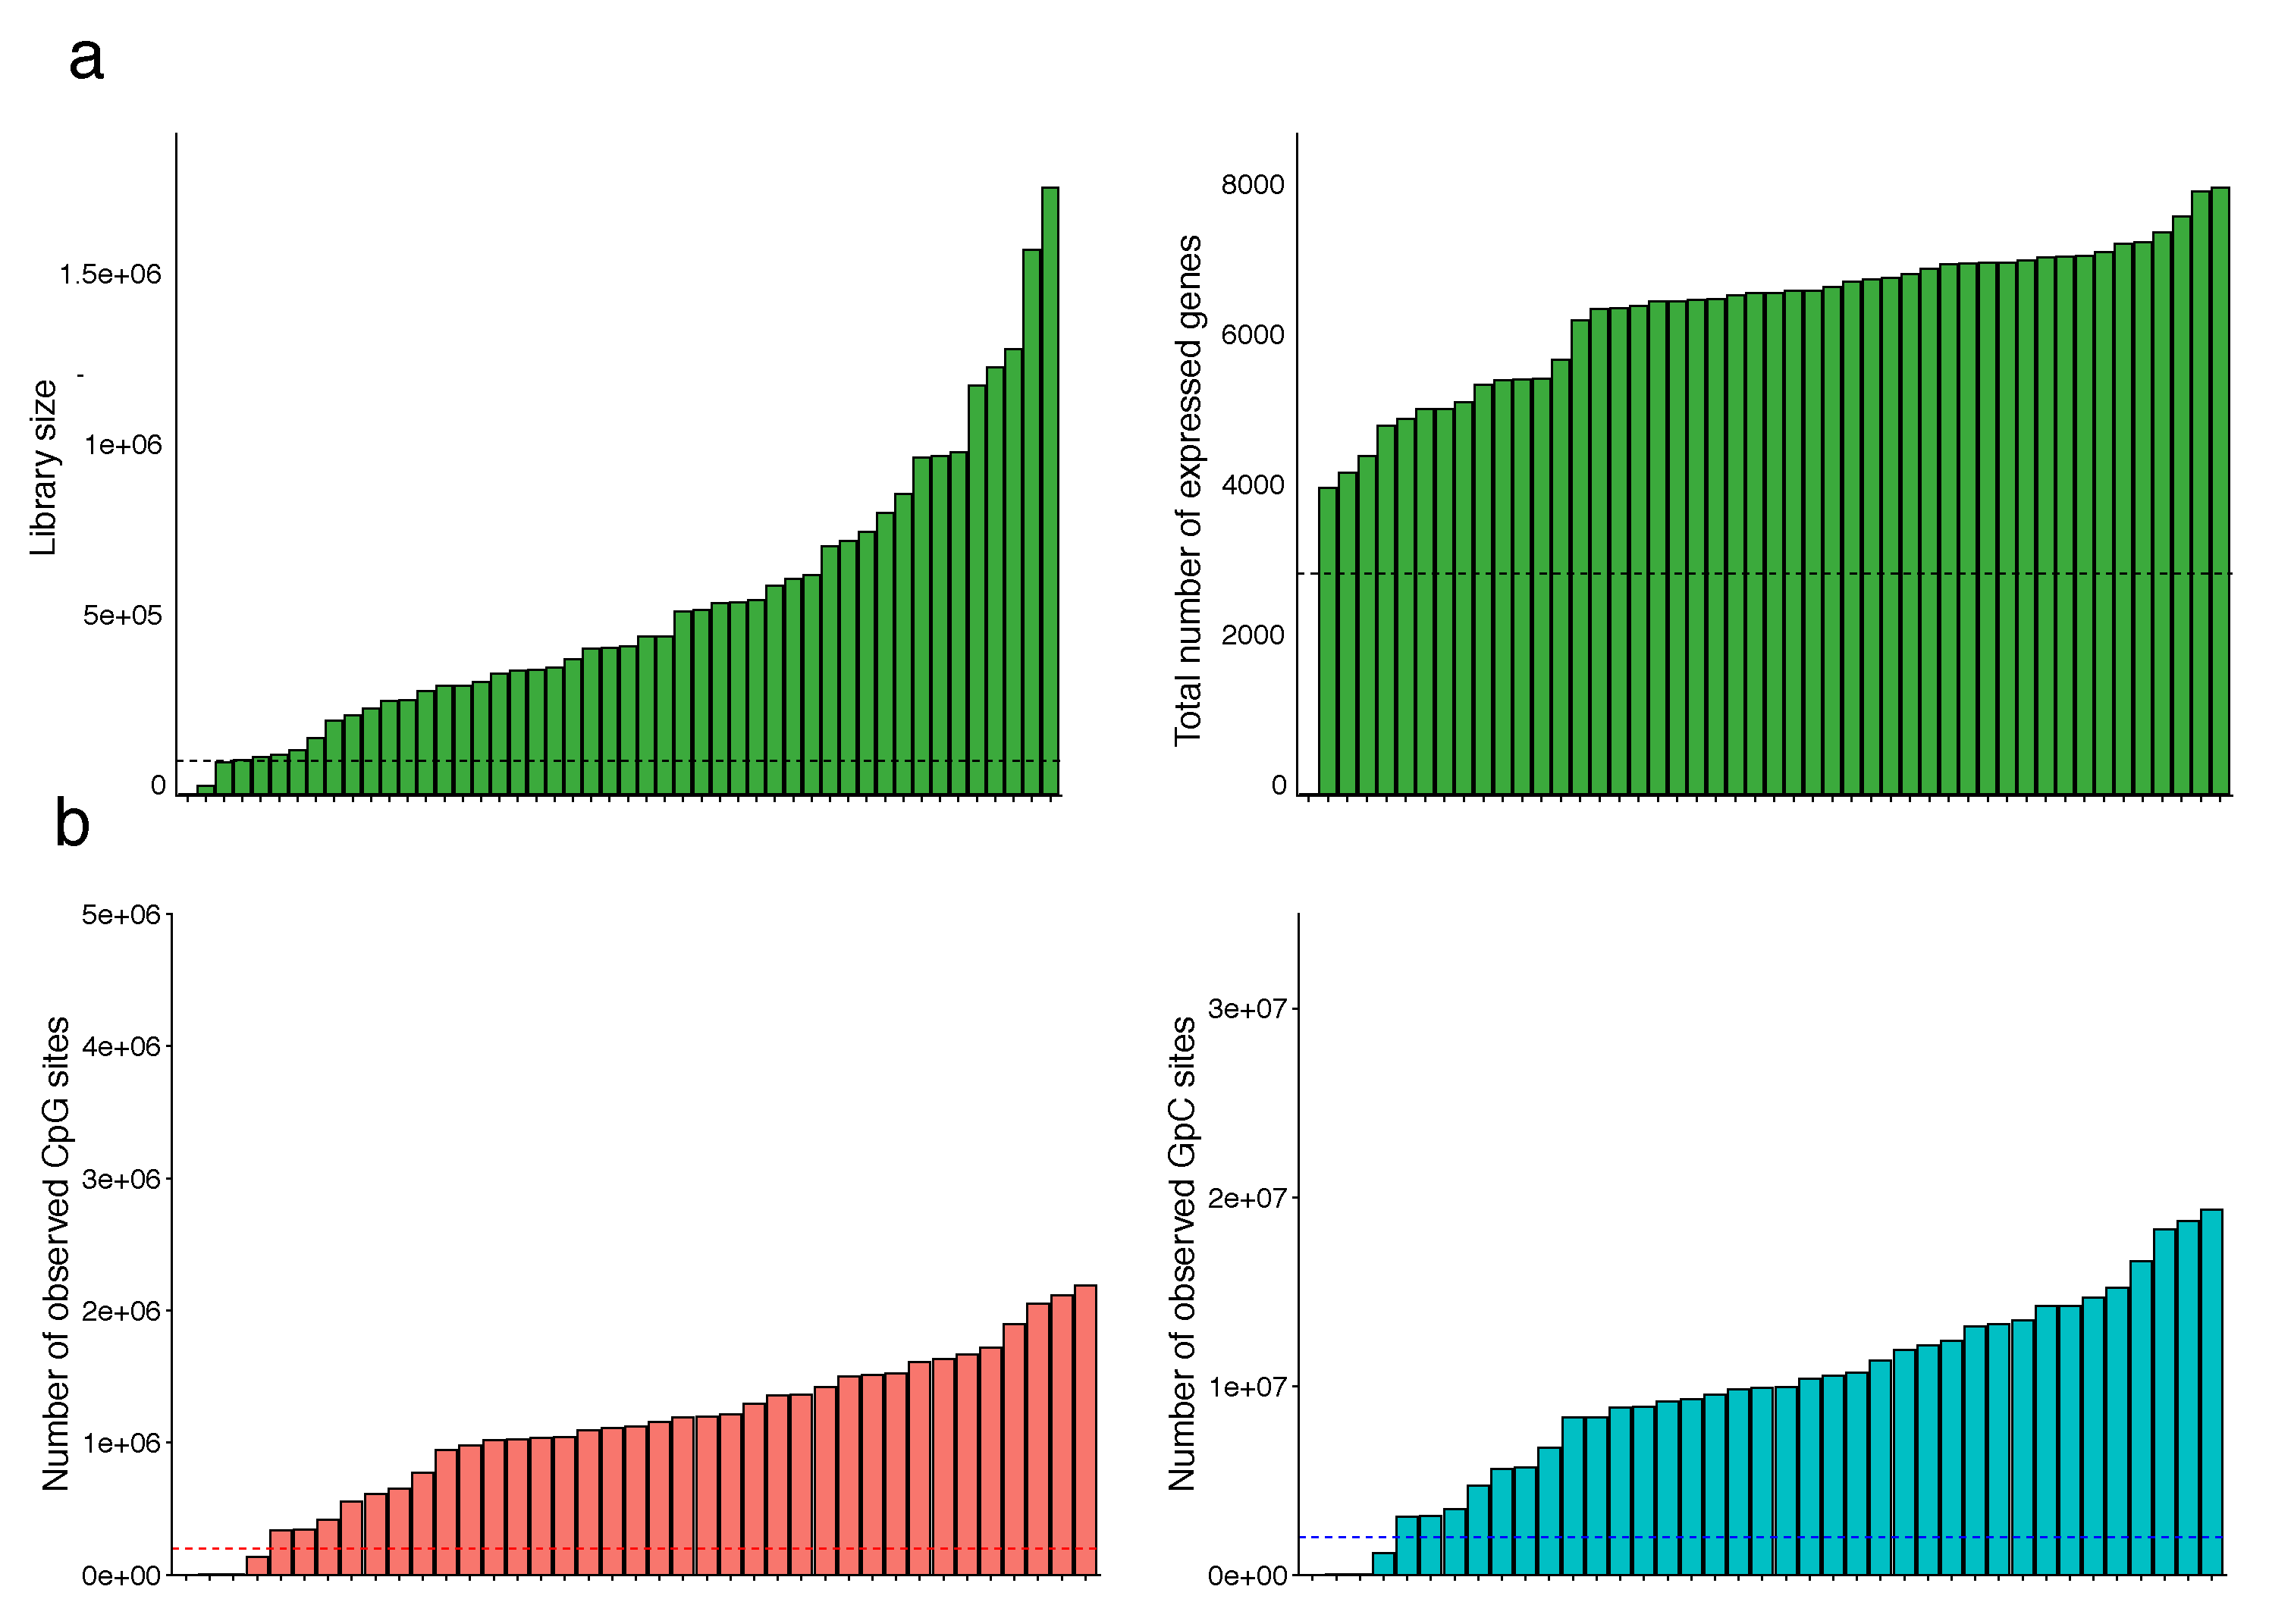
\includegraphics[width=0.8\linewidth]{scNMT_EB_QC}
% 	\caption[]{Quality control statistics on the 43 embryoid body cells. (a) number of aligned RNA reads per cell (left) and number of expressed genes (right). (b) Number of CpG sites (DNA methylation) observed. (c) Number of GpC sites (chromatin accessibility) observed. Dashed lines indicate binary thresholds, such that cells below the threshold are excluded for the downstream analysis.}
% 	\label{fig:scnmt_eb_qc}
% \end{figure}


\begin{figure}[H]
	\centering
	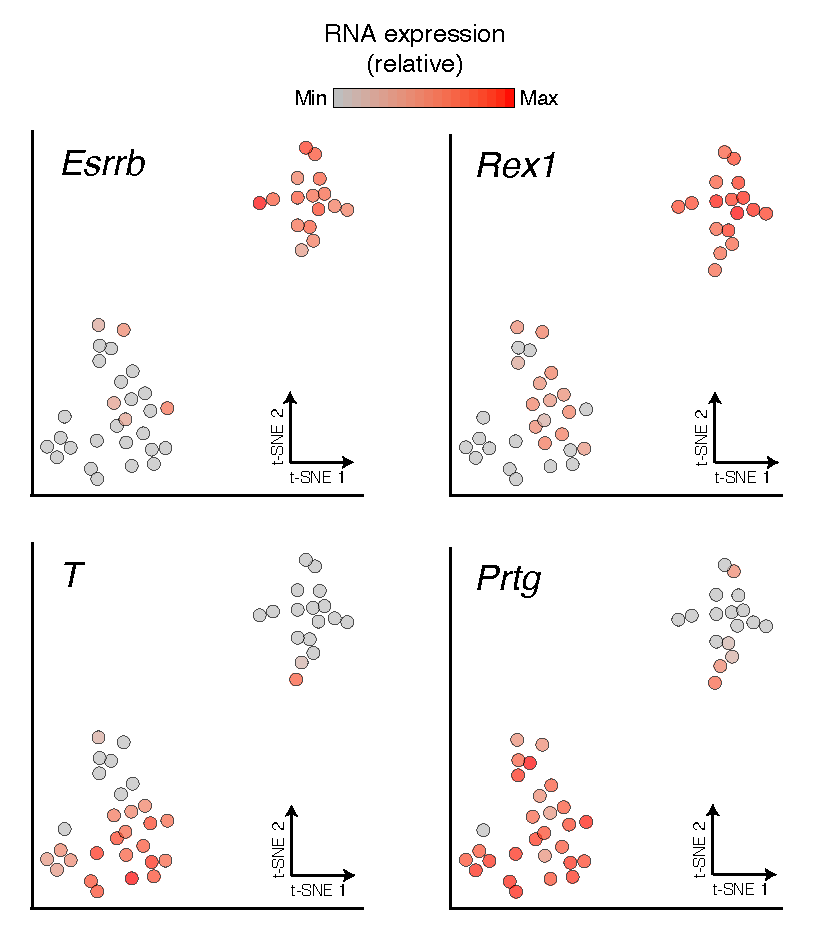
\includegraphics[width=1.00\linewidth]{scNMT_EB_RNA}
	\caption[]{\textbf{t-SNE representation of the RNA expression profiles for the embryoid body cells}.\\
	The scatter plots show a t-SNE \cite{vanDerMaaten2008} representation of the EB data. Cells are coloured based on expression of pluripotency factors (top) and differentiation markers (bottom). }
	\label{fig:scnmt_eb_rna}
\end{figure}

Next, we tested for locus-specific associations between pairwise combinations of molecular layers (correlation across cells, \Cref{fig:scnmt_eb_correlations}).\\
First, considering correlations between DNA methylation and RNA expression, we identified a majority of negative associations, reflecting the known relationship between these two layers. In contrast, we obtained largely positive associations between chromatin accessibility and RNA expression, mainly in promoters, p300 binding sites and super enhancer regions. Finally, we found mostly negative associations between DNA methylation and chromatin accessibility. This confirms the expected direction of association between molecular layers, as reported in bulk studies.\\
As an illustrative example, we display the \textit{Esrrb} locus, a gene involved in early development and pluripotency \cite{Papp2012}. A previous study \cite{Angermueller2016}, identified a super enhancer near the gene that showed a high degree of correlation between DNA methylation and RNA expression changes. In our study, we find \textit{Esrrb} to be expressed primarily in the pluripotent cells, consistent with its role in early development. When examining the epigenetic dynamics of the corresponding super enhancers, we observe a strong negative correlation between DNA methylation and RNA expression, thus replicating previous findings. Additionally, we observe a strong negative relationship between DNA methylation and chromatin accessibility, indicating the two epigenetic layers are tightly coupled.

\begin{figure}[H]
	\centering
	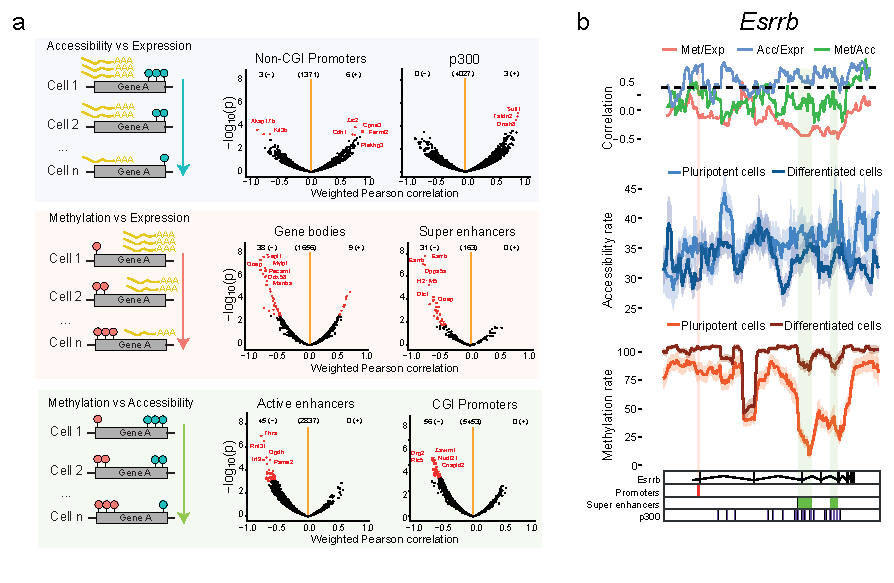
\includegraphics[width=1.0\linewidth]{scNMT_EB_correlations}
	\caption[]{
	\textbf{scNMT-seq enables the discovery of novel associations between transcriptomics and epigenetics at individual loci.}\\ 
	(a) Illustration for the correlation analysis, which results in one association test per locus (across cells). \\
	(b) Pearson correlation coefficient (x-axis) and log10 p-value (y-axis) from association tests between different molecular layers, stratified by genomic contexts. Significant associations (FDR<0.1), are highlighted in red.\\
	(c) Zoom-in view of the \textit{Esrrb} gene locus. Shown from top to bottom are: Pearson correlation between each pair of molecular layers. Accessibility (blue) and methylation (red) profiles shown separately for pluripotent and differentiated sub-populations; mean rates (solid line) and standard deviation (shade) were calculated using a running window of 10kb with a step size of 1kb. Track with genomic annotations highlighting the position of regulatory elements.
	}
	\label{fig:scnmt_eb_correlations}
\end{figure}


% \subsection{Inference of non-linear chromatin accessibility profiles at single nucleotide resolution}

% A clear advantage of scNMT-seq is the high resolution of the chromatin accessibility readouts, namely a binary output for each observed GpC dinucleotide. As illustrated in \Cref{fig:scnmt_pseudobulk_profiles}, GpC accessibility measurements rate extremely dynamic and display complex oscillatory patterns, likely due to presence of nucleosomes. This makes our approach of quantifying rates over a fixed genomic window not appropriate to capture the complexity of accessibility data. Therefore, we next attempted to exploit this high-resolution information to infer non-linear chromatin accessibility profiles at individual promoters.\\
% The approach we followed is based on BPRMeth \cite{Kapourani2018}, a generalized linear regression model with Gaussian basis functions, coupled with a Bernoulli likelihood. A model was fit for every gene and every cell, provided enough coverage (at least 10 GpC sites observed per gene across 40\% of cells). Examples of inferred regression patterns are shown below:

% \begin{figure}[H]
% 	\centering
% 	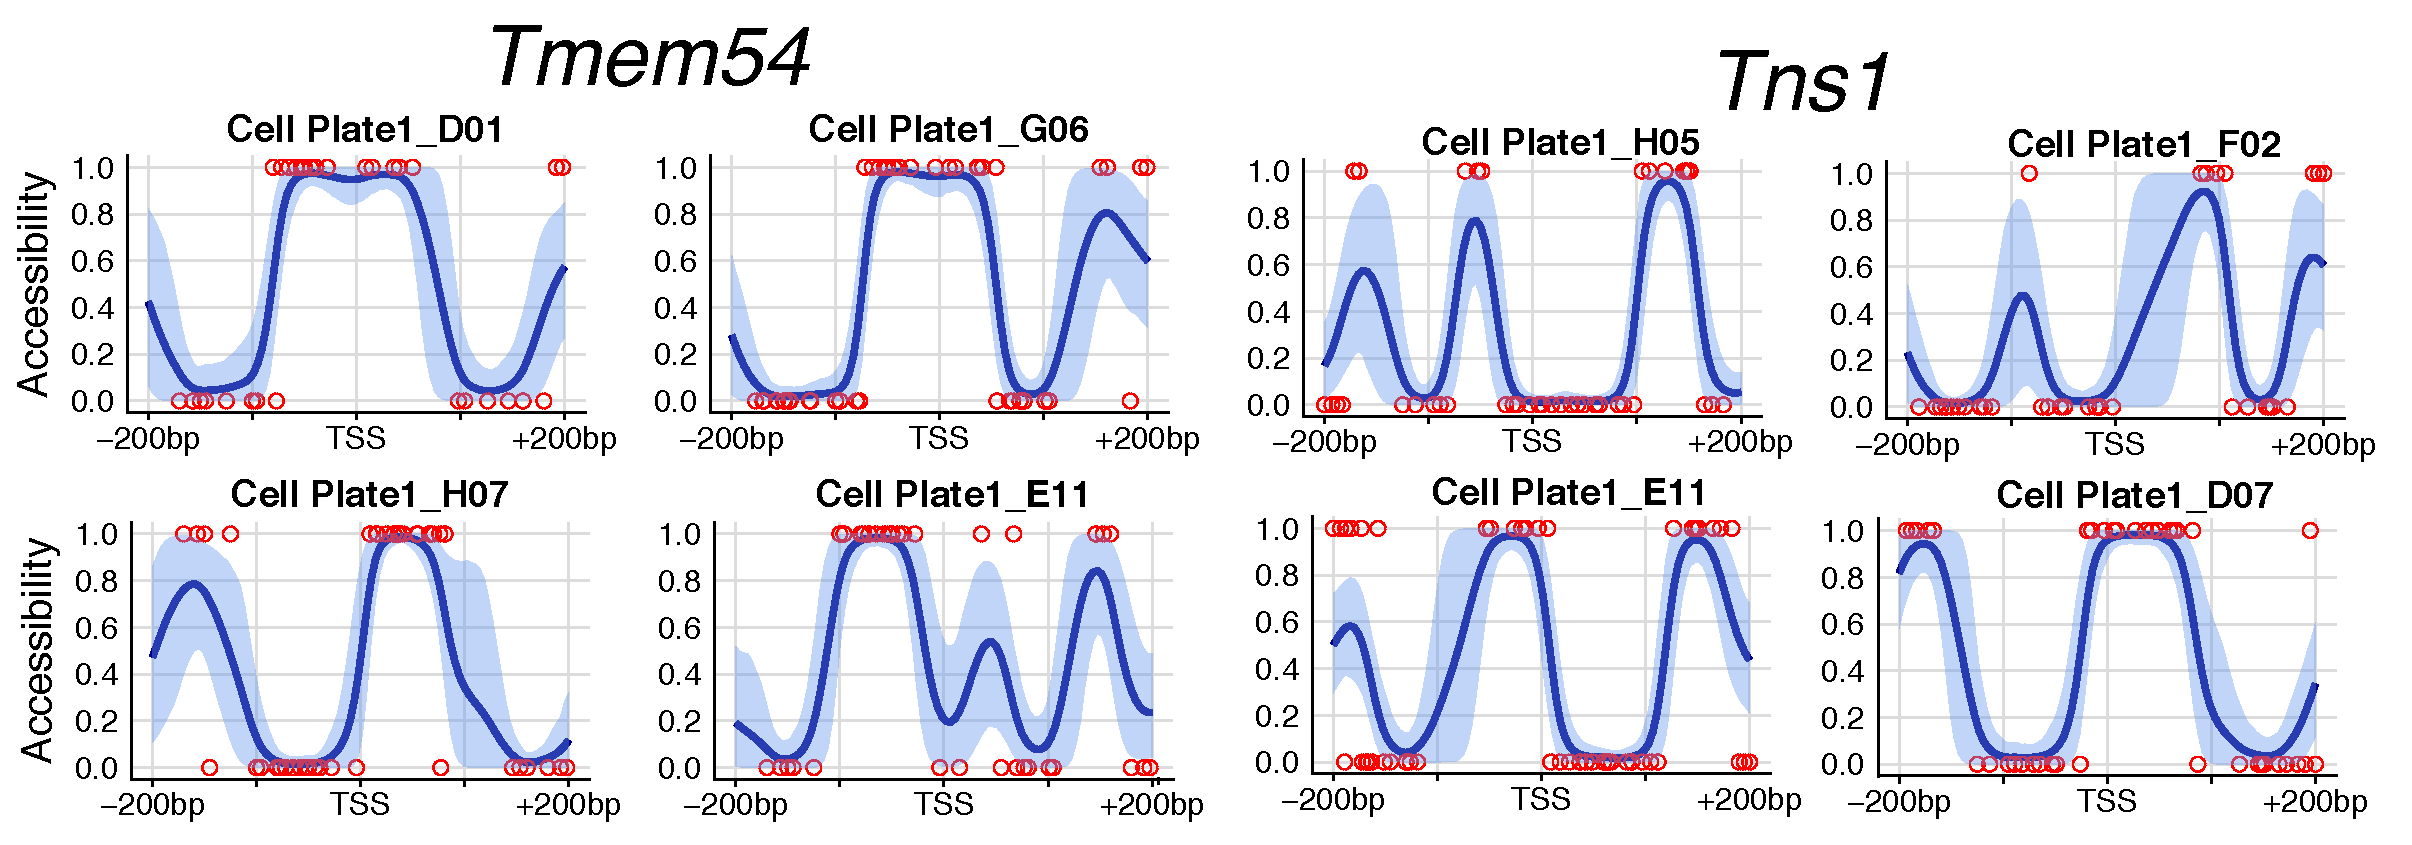
\includegraphics[width=0.9\linewidth]{scNMT_profiles_examples}
% 	\caption[]{\textbf{Illustrative examples of single-cell accessibility profiles around the transcription start site}.\\
% 	Shown are representative profiles for two genes, \textit{Tmem54} and \textit{Tns1}. Each panel corresponds to separate cell. The y-axis displays the binary GpC accessibility values, with 1 being accessibility and 0 inaccessible. The x-axis displays the genomic region around the TSS (200bp upstream and downstream). The blue area depicts the inferred (non-linear) accessibility profile using the BPRMeth model \cite{Kapourani2018}.}
% 	\label{fig:scnmt_profiles_examples}
% \end{figure}

% As a simple validation, we verified that highly expressed genes show characteristic patterns of nucleosome depleted regions around the TSS, whereas lowly expressed genes show low levels of chromatin accessibility:

% \begin{figure}[H]
% 	\centering
% 	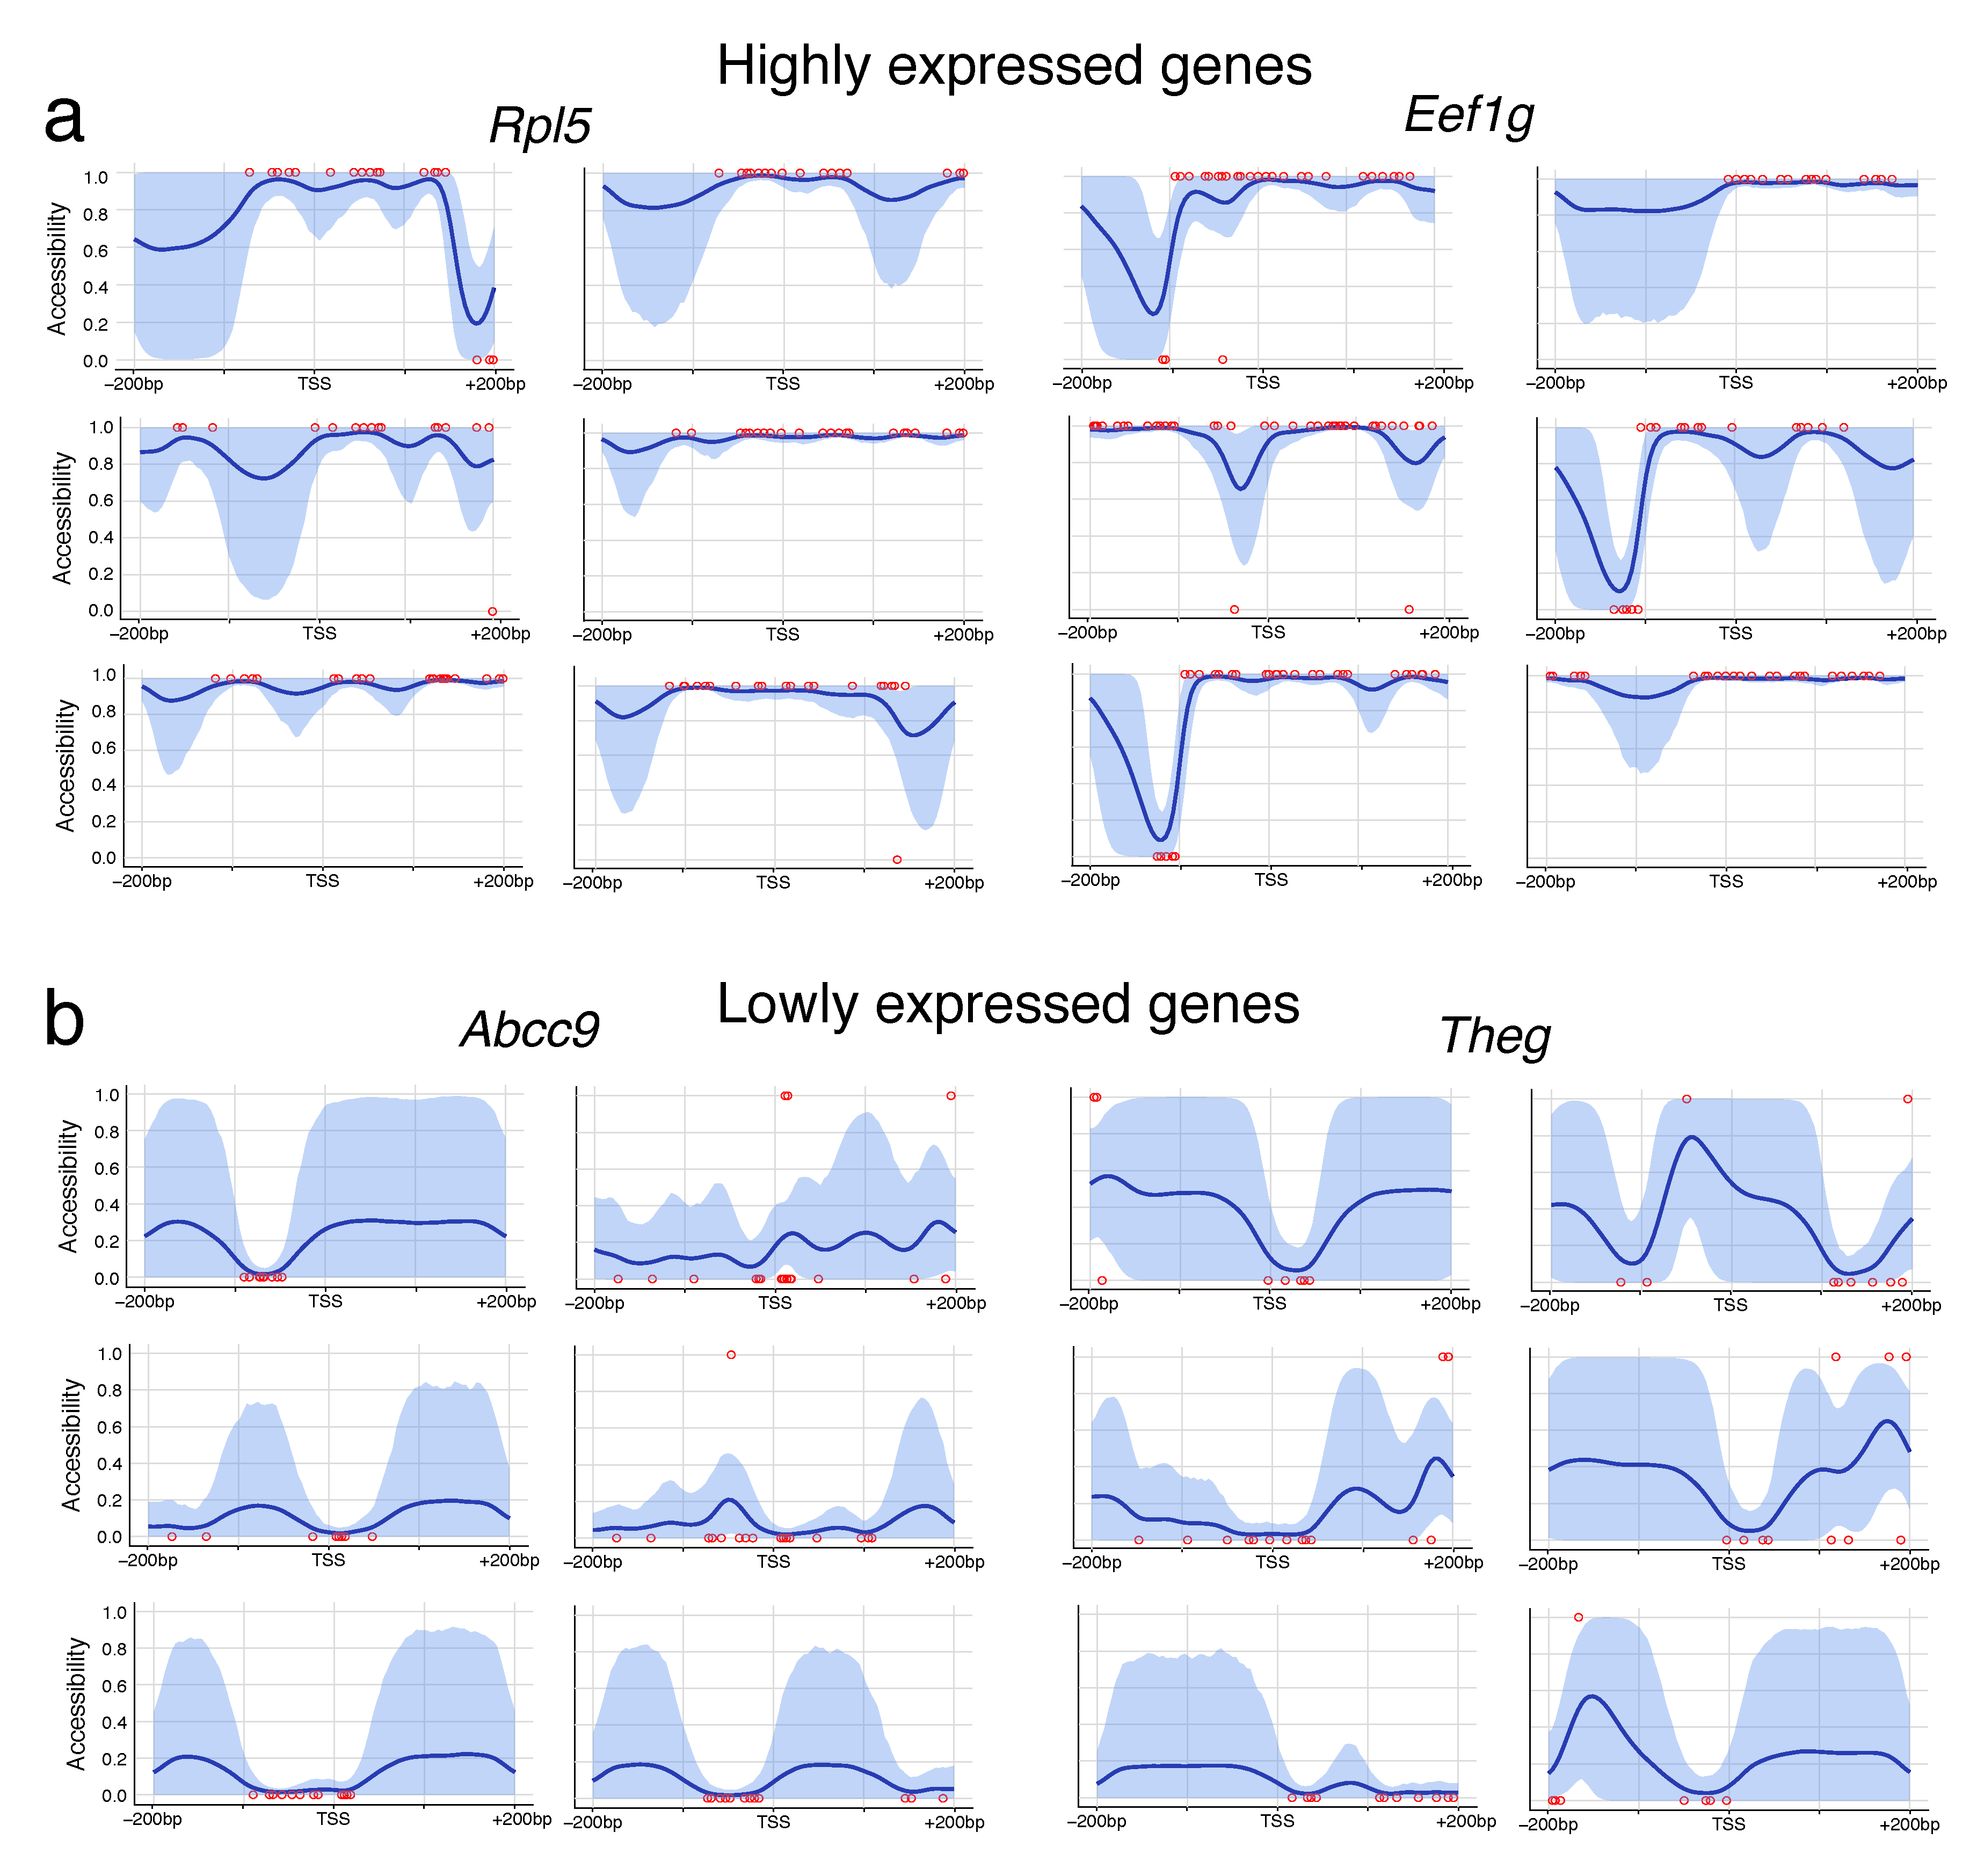
\includegraphics[width=0.9\linewidth]{scNMT_profiles_expr}
% 	\caption[]{\textbf{Single-cell accessibility profiles of representative genes with high and low expression levels.}\\
% 	Shown are \textit{Rpl5} and \textit{Eef1g} (high expression levels, top); \textit{Abcc9} and \textit{Theg} (low expression levels, bottom). Each panel corresponds to a separate cell. Axis are the same as in \Cref{fig:scnmt_profiles_examples}. }
% 	\label{fig:scnmt_profiles_highexpr}
% \end{figure}

% Using this statistical framework we attempted to link the heterogeneity in chromatin accessibility with the variability in RNA expression.\\
% A challenge of this computational representation is defining a unidimensional statistic that summarises the heterogeneity across cells (as the variance statistic in conventional rates), which can be in turn correlated with summary statistics from the RNA expression. The approach we followed here is to cluster cells (per gene) based on the similarity of the accessibility profiles, using a finite mixture model with an expectation-maximisation algorithm. The optimal number of clusters was estimated using a Bayesian Information Criterion.\\
% After model fitting, we considered the number of clusters as a proxy for accessibility heterogeneity, the rationale being that homogeneous genes will be grouped in a single cluster, while heterogeneous genes will contain a higher number of clusters. The result of the analysis is shown below:\\

% \begin{figure}[H]
% 	\centering
% 	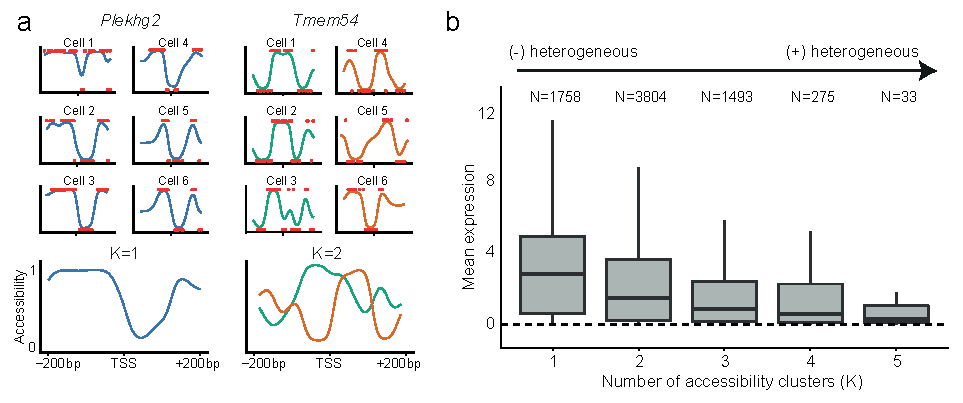
\includegraphics[width=0.9\linewidth]{scNMT_profiles_clusters}
% 	\caption[]{
% 	\textbf{Clustering chromatin accessibility profiles at gene promoters}. \\
% 	(a) Accessibility profiles are fitted for each cell and gene using 200 bp windows around the TSS. Then, a clustering step is applied for each gene and the most likely number of clusters is estimated using a Bayesian Information Criterion. Genes with higher numbers of clusters correspond to genes with increased heterogeneity compared to genes with small numbers of clusters.\\
% 	(b) Relationship between heterogeneity in the accessibility profile (x-axis) and average gene expression (across cells, y-axis).
% 	}
% 	\label{fig:scnmt_profiles_clusters}
% \end{figure}

% Genes with homogeneous accessibility profiles (fewer clusters) are associated with higher average expression levels. This includes genes with housekeeping functions, which are known to display highly conserved epigenetic features \cite{She2009}. In contrast, genes with heterogeneous accessibility (more clusters) are associated with lower expression levels. Interestingly, these genes are enriched for bivalent domains, containing both active H3K4me3 and repressive H3K27me3 histone marks (\Cref{fig:scnmt_profiles_histones}). As reported in previous studies, bivalent chromatin is normally associated with lowly-expressed genes that are poised for activation upon cell differentiation, thus playing a fundamental role in pluripotency and development \cite{Vastenhouw2012,Bernstein2006}

% \begin{figure}[H]
% 	\centering
% 	\includegraphics[width=0.80\linewidth]{scNMT_profiles_histones}
% 	\caption[]{\textbf{High levels of heterogeneity in chromatin accessibility are associated with the presence of bivalent histone marks (H3K4me3 and H3K27me3)}.\\
% 	Proportion of gene promoters marked with different sets of histone mark combinations (y-axis), stratified by number of accessibility clusters (x-axis)
% 	}
% 	\label{fig:scnmt_profiles_histones}
% \end{figure}


\subsection{Exploration of epigenome and transcriptome connections}

The use of single-cell technologies has permitted the unbiased study of continuous trajectories by computationally reconstructing the \textit{pseudotemporal} dynamics from the molecular profiles \cite{Trapnell2014,Haghverdi2016,Saelens2018}. A novel opportunity unveiled by the introduction of single-cell multi-modal technologies is the study of epigenetic dynamics along trajectories inferred from the transcriptome. To explore this idea, we applied a diffusion-based pseudotime method \cite{Haghverdi2016} to the EB data set, using the RNA expression of the 500 genes with highest biological overdispersion \cite{Lun2016b}. The first diffusion component was used to reconstruct a pseudotemporal ordering of cells from pluripotent to differentiated states:

\begin{figure}[H]
	\centering
	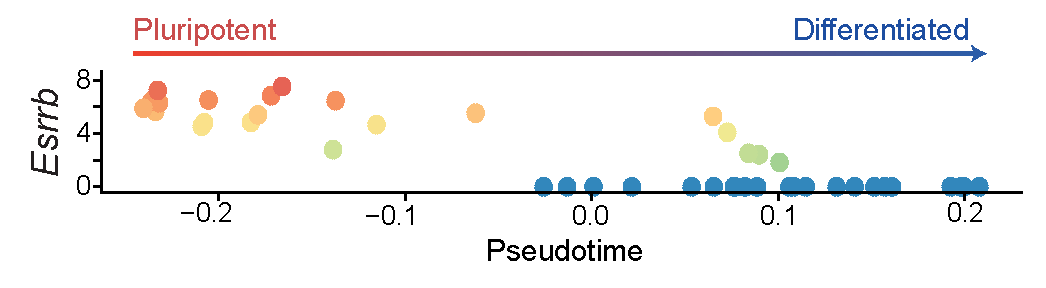
\includegraphics[width=0.75\linewidth]{scNMT_pseudotime}
	\caption[]{\textbf{Reconstruction of developmental trajectory in embryoid body cells from the RNA expression data}.\\
	Each dot corresponds to one cell. The y-axis displays expression of \textit{Esrrb}, a canonical pluripotency marker, and the x-axis shows the position of the cells in the first diffusion component.}
	\label{fig:scnmt_pseudotime}
\end{figure}


Using the pseudotime reconstruction we investigated whether the strength of association between molecular layers (as calculated in \Cref{fig:scNMT_correlations_acrossgenes}) are affected along the developmental trajectory. To do this, we correlated the correlation coefficient across genes between each pair of molecular layers (one value per cell) versus the pseudotime position (\Cref{fig:scnmt_pseudotime_coupling}). Importantly, this analysis is possible by the continuous nature of single-cell data and by the ability of scNMT-seq to profile three molecular layers at the same time.\\
We observe that for DNA methylation and chromatin accessibility, the negative correlation coefficients decreases in important regulatory genomic contexts (\Cref{fig:scnmt_pseudotime_coupling}), such that pluripotent cells have a notably weaker methylation-chromatin coupling than differentiated cells. This suggests that the strength of regulation between molecular layers can be altered during cell fate decisions.

\begin{figure}[H]
	\centering
	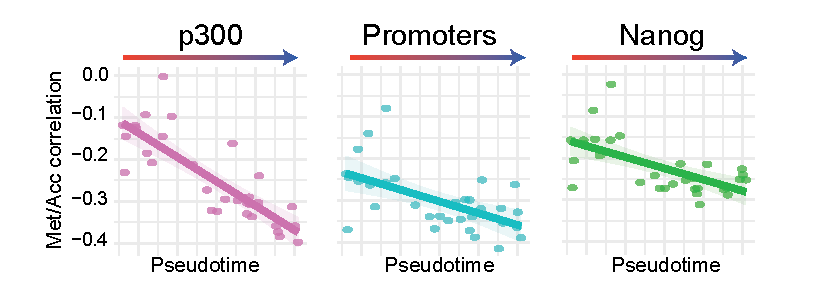
\includegraphics[width=0.9\linewidth]{scNMT_pseudotime_coupling}
	\caption[]{\textbf{Developmental trajectory is associated changes in methylation-accessibility coupling.}\\
	Shown is the location of each cell in pseudotime (x-axis) and the corresponding Pearson correlation coefficients between methylation and accessibility (y-axis) in three different genomic contexts with regulatory roles.
	}
	\label{fig:scnmt_pseudotime_coupling}
\end{figure}

\section{Conclusions and open perspectives}

In this Chapter I have introduced single-cell nucleosome, methylation and transcriptome sequencing (scNMT-seq), an experimental protocol for the genome-wide profiling of RNA expression, DNA methylation and chromatin accessibility in single cells. This novel assay is an important step forward in the field of single-cell multi-modal sequencing. Yet, as with other protocols, the technology is still in a very early stage and numerous developments are expected to occur in the next years. Some lines of research that I believe are important to improve scNMT-seq are the following:

\begin{itemize}

	\item \textbf{Scalability}: scRNA-seq protocols are reaching the astonishing numbers of millions of cells per experiment. This contrasts with the limited cell numbers achieved in current multi-modal assays, including scNMT-seq \cite{Cao2019,Cao2018,Guo2017}. As in scRNA-seq, the maturation of multi-modal techniques will display a trade-off between sensitivity and scalability \cite{Chappell2018}. scNMT-seq already provides high-resolution measurements, thus effort should be placed on making the protocol more scalable, which can be achieved by a series of technical improvements. First, barcodes are currently added at the end of the protocol, which limits cell numbers to the size of the plate. As in droplet-based methods or combinatorial indexing methods, adding the barcodes at the start of the protocol would enable the simultaneous processing of multiple pools of samples \cite{Dey2015,Mulqueen2018}. Second, the physical separation of mRNA from genomic DNA is performed at the beginning of the protocol, one cell at a time. Given that it is a time-consuming and expensive process, this step should be performed after pooling \cite{Dey2015}. Finally, albeit sequencing costs are decreasing \cite{Svensson2018}, the sequencing of scNMT-seq libraries remains expensive due to genome-wide coverage. Hence, I anticipate that efforts to decrease the library size by a pre-selection of the genetic material will be indispensable. Examples of such strategies are the digestion by restriction enzymes as in RRBS \cite{Guo2013}, an initial round of ATAC protocol to select open chromatin \cite{Spektor2018} or the pull-down of specific genomic regions using capture probes.

	\item \textbf{Imputation of missing epigenetic data}: because of the low amounts of starting material, single-cell methylation protocols are limited by incomplete CpG coverage \cite{Angermueller2017}. This becomes even more pronounced in scNMT-seq where almost $\approx$ 50\% of CpG dinucleotides are removed to avoid technical biases (see \Cref{section:scnmt_coverage}). Nonetheless, as discussed in \Cref{section:scnmt_protocol}, an important advantage of bisulfite approaches is that missing data can be discriminated from inaccessible chromatin (unlike in scATAC-seq). Therefore, the imputation of DNA methylation data will likely be a critical step to enable genome-wide analysis. Most of the imputation methods developed for bulk data are unsuccesful because they do not account for cell-to-cell variability \cite{Angermueller2017}. A successful single-cell strategy based on deep learning has been proposed (DeepCpG \cite{Angermueller2017}), but is a complex model that is difficult to train and does not scale to large datasets. Faster and accurate Bayesian approaches have also been considered (Melissa \cite{Kapourani2018b}), albeit the model is restricted to a small feature set and cannot perform genome-wide imputation.

	\item \textbf{Adding more molecular layers}: scNMT-seq can be adapted both experimentally and computationally to profile additional molecular layers. From the computational side, one could exploit the sequence information in the libraries to infer copy number variation or single nucleotide variants \cite{Poirion2018,Fan2018,McCarthy2018,Enge2017}. This approach has been successful at delineating the clonal substructure of somatic tissues and at tracking mutational signatures in cancer tissues. In addition, the full length transcript information enables the quantification of splice variants\cite{Huang2017}, allele-specific fractions \cite{Deng2014} and RNA velocity information \cite{LaManno2018}. From the experimental side, scNMT-seq could be combined with novel single-cell assays that quantify protein expression \cite{Stoeckius2017}, transcription factor binding \cite{Moudgil2019} and histone modifications \cite{Kaya-Okur2019}.

	% \item \textbf{Denoising}: in scNMT-seq the CGC positions (27\%) suffer from off-target effects of the GpC methylase \cite{Kelly2012}. In this work we have excluded those measurements to avoid undesired technical variation. Yet, no attempts have been carried to quantify this effect. If small enough, one could denoise the resulting CpG measurements by machine learning techniques that use sequence context information.
	% %The readouts from bisulfite sequencing are very sensitive \cite{XX}. 

	\item \textbf{Long reads}: the scNMT-seq libraries that were generated for this study contained short reads (75bp) that do not provide sufficient information about the regional context of the individual DNA molecule. By sequencing NOMe-seq libraries with long-read nanopore sequencing technology \cite{Lee2018} showed that one can obtain phased methylation and chromatin accessibility measurements and structural changes from a single assay. This approach could potentially unveil a more comprehensive understanding of the epigenome dynamics and its regulatory role on RNA expression.

\end{itemize}


% In conclusion, we have shown that the use of non-linear methods for summarising NOMe-seq accessibility data can yield novel insights into the chromatin organisation, nucleosome positioning and the consequent regulation of gene expression. Yet, we acknowledge that this novel computational methodology needs to be further validated using other datasets, and some improvements need to be implemented in order to ensure that robust biological signal can be extracted from single-cell studies. First, the use of faster inference frameworks, which has been implemented in the new version of the software \cite{Kapourani2018}. Second, the method requires a large number of measurements for an accurate regression. In this study we used relatively lenient thresholds and only $\approx$25\% genes passed coverage filtering. An attempt to improve this could be the use of Bayesian methods that simultaneously cluster and fit the regression model, effectively leveraging information about the similarity between individual cells \cite{Kapourani2018b}. Finally, one could aim at learning a joint model with DNA methylation and chromatin accessiblity to provide an extra layer of multi-modal information.

